\Chapter{A MySQL Connector}

\Section{Ismertető}
A MySQL Connector egy MySQL alapú driver JDBC, ODBC, és .NET rendszerek számára. Lehetővé teszi, hogy a fejlesztők adatbázis alkalmazásokat írjanak a támogatott nyelveken. Ezen kívül egy natív C könyvtár teszi lehetővé, hogy a MySQL-t közvetlenül beágyazhassák az alkalmazásaikba.
MySQL által fejlesztett driver -ek:
ADO.NET, ODBC, JDBC, Node.js, Python, C++, C és C API a a klienshez. 
A MySQL közösség által fejlesztetek:
PHP, Perl, Ruby, C+ Wrapper.

*https://www.mysql.com/products/connector/

\Section{A Connector/C++ használata}

Az alábbi weboldalról letöltött állományokat használtam:\newline
https://dev.mysql.com/downloads/connector/cpp/
\begin{itemize}
\item Linux - Generic
\item All
\item Linux - Generic (glibc 2.12) (x86, 64-bit), Compressed TAR Archive
\end{itemize}

Letöltés után kicsomagoljuk. A tartalma egy include és egy lib64 mappa. Az include mappa tartalmát a usr/include könyvtárba másoljuk, a lib64 -ét pedig az usr/lib64 mappába.

Ezután szükség lesz egy külön felhasználóra amellyel a program csatlakozni fog a szerverünkre. Ezt megtehetjük a Workbench alkalmazásban.
\begin{python}
CREATE USER 'newuser'@'localhost' IDENTIFIED BY 'password';
\end{python}

\Section{Első program}

Hozzunk létre egy \texttt{connectortest.cpp} nevű fájlt.
Szükséges osztályok létrehozása:
\begin{cpp}
sql::Driver *driver;
sql::Connection *con;
sql::Statement *stmt;
sql::ResultSet *res;
sql::PreparedStatement *pstmt;
\end{cpp}
Csatlakozás a szerverhez és adatbázis kiválasztása:
\begin{cpp}
driver = get_driver_instance();
con = driver->connect("tcp://192.168.0.43:3306", "program", "a");
con->setSchema("thesis");
\end{cpp}
Utasítás létrehozása SQL parancsból:
\begin{cpp}
pstmt = con->prepareStatement("SELECT * FROM T3");
\end{cpp}
Az utasítás elküldése a szervernek. Ez a sor maga a lekérdezés, itt tudjuk mérni annak idejét is.
\begin{cpp}
res = pstmt->executeQuery();
\end{cpp}
Az eredményt a szemléltetett módon lehet kiolvasni:
\begin{cpp}
 while (res->next())
      cout << res->getInt("c1p3") << "\t" << res->getInt("c2") << "\t"
           << res->getInt("c3") << "\t" << res->getInt("c4") << "\t"
           << res->getInt("fk_p1_p3") << "\t" << res->getInt("fk_p2_p3") 
           << endl;
\end{cpp}


Lekérdezés után fontos törölni az eredményhalmazt és az elkészített utasítást, ugyanis ezek memóriát foglalnak, és több lekérdezés esetén a lekérdezés halmaz megtöltheti a teljes memóriát is. 
\begin{cpp}
    delete res;
    delete pstmt;
\end{cpp}


Futtatáshoz és fordításhoz a következő parancsokat használhatjuk: 
\begin{python}
g++ -D_GLIBCXX_USE_CXX11_ABI=0 connectortest.cpp -o connectortest.out -lmysqlcppconn
./connectortest.out
\end{python}

\Chapter{Párhuzamosítási lehetőségek}

\Section{Az OpenCL nyelv}

Open Computing Language egy keretrendszer amely lehetőséget ad olyan programok írására amelyek különböző platformokon is futtathatóak.
Az OpenCL meghatároz egy programozási nyelvet az eszközök és API-k számára a platformok vezérléséhez és a számítások végrehajtásához az eszközökön. Szabványos interfészt biztosít a párhuzamos számításokhoz, melyhez adatalapú és feladatalapú párhuzamosítást használ.

Fontos észrevenni, hogy az OpenCL natív módon képes beszélni az eszközök nagy részével, ez nem azt jelenti, hogy a kód optimálisan fog futni. Ugyanis különböző Cl eszközök különböző funkciókkal vannak ellátva. Gyártó specifikus kiterjesztések elkerülésével a kód hordozható lesz, de nem sebesség optimális.

\begin{figure}[h!]
\centering
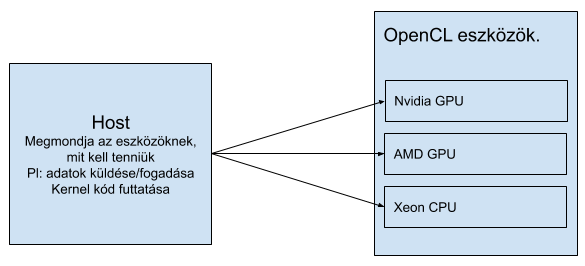
\includegraphics[width=\textwidth]{images/opencl.png}
\caption{OpenCL}
\label{fig:opencl}
\end{figure}

A következő esetekben a GPU-t érdemes használni.
\begin{itemize}
\item Gyors permutáció: Az eszközök gyorsabban mozgatáják a memóriát mint a Host.
\item Adat átváltás: Egyik formátumról másikra.
\item Numerikus gyorsítás: Az eszközök gyorsabban számolnak nagyobb adatdarabokkal mint a Host.
\end{itemize}
Jelen esetben a Host egy asztali számítógép.
Számítási eszközei: CPU, GPU, FPGA, DSP.
A számítási egységek: a magok száma
Elemek feldolgozása: ALU-k magunként.

OpenCL használata mellett szükségtelen gondolkozni azon, hogy pontosan mi is végzi el a számításokat. Ugyanis az OpenCL modelljének illeszkedése egy adott hardverhez, a gyártók feladata.

\begin{table}[h!]
\centering
\caption{CPU-k és GPU-k összehasonlítása}
\medskip
\label{tab:cpuvsgpu}
\begin{tabular}{|p{7cm}|p{7cm}|}
\hline
Alacsony számítási sűrűség & Magas számítási sűrűség \\
\hline
Komplex logikai vezérlő & Magas számítási és memória-hozzáférés \\
\hline
Nagy caches &   \\
\hline
Optimalizált a soros műveletekre.
\begin{itemize}
	\item Kevesebb végrehajtási egység (ALU).
	\item Magas órajel sebesség.
\end{itemize} & Beépített párhuzamos műveletek.
\begin{itemize}
	\item Sok párhuzamos végrehajtási egység (ALU).
	\item A grafika a párhuzamosság legismertebb esete.
\end{itemize} \\
\hline
Shallow pipelines <30 stages & Deep pipelines több száz szakasz \\
\hline
Alacsony késleltetési tolerancia & Magas áteresztőképesség, Magas áteresztőképesség \\
\hline
Az újabb CPU-k több párhuzamosításra képesek & Újabb GPU-k
\begin{itemize}
	\item Jobb áramlást vezérlő logika
	\item Scatter/Gather Memory Access
	\item Már nem egyirányúak a pipeline-ok
\end{itemize} \\
\hline
\end{tabular}
\end{table}

\SubSection{Az OpenCL elemei}
\begin{itemize}
\item Globális memória: Minden eszközzel meg van osztva, de lassú. A kernel hívások között perzisztens. 
\item Konstans memória: Gyorsabb a globálisnál, szűrő paraméterek megadására használják.
\item Lokális memória: Minden számási egység számára privát, de megosztott a feldolgozó elemek között.
\item Privát memória: Gyorsabb a lokálisnál, minden feldolgozó elemnek van.
\end{itemize} 
A konstans, lokális és privát memóriába nem lehet adatokat menteni úgy, hogy más kernel használhassa majd azt




\Section{Az OpenCL telepítése}

A megfelelő működéshez az első lépést már a rendszer telepítésénél megtettem amikor a non-free avagy az nvidia eredeti drivernének a telepítését választottam.
ezen kívül a következő csomagokra volt szükség: 

\begin{python}
$ sudo pacman -S opencl-headers
$ sudo pacman -S opencl-nvidia
$ sudo pacman -S cuda
$ sudo pacman -S ocl-icd
\end{python}

\Section{Az OpenCL használata}

\Chapter{Megvalósítás}

\Section{Bevezetés}

Az ötletet egyik legjobban hátráltató dolog az adatbázis elérése. Ahhoz, hogy hozzá férjünk az adatokhoz szükség van a Connectorra, amely egy teljes lekérdezést végezve vissza tér a táblával. Ezen adatokat át kell másolni egy a tábla felépítését reprezentáló strúktúrából álló vektorba.



